\documentclass[tikz,border=12pt]{standalone}
\usepackage{amsmath,amssymb}
\usetikzlibrary{calc,arrows.meta}

\begin{document}
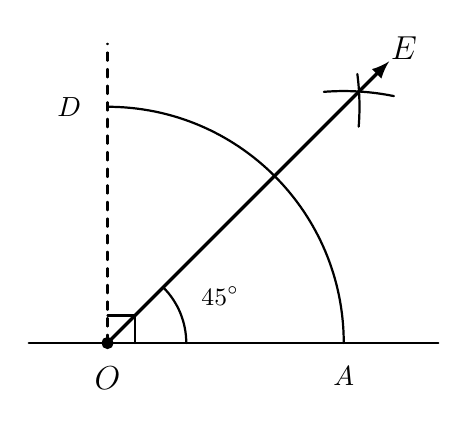
\begin{tikzpicture}[>=latex, line cap=round, line join=round]
  % Parameters
  \def\r{3.0}     % Radius of base quadrant arc
  \def\R{3.2}     % Radius of bisector arcs
  
  % Baseline
  \draw[thick] (-1.0, 0) -- (4.2, 0);

  % Vertex O
  \coordinate (O) at (0, 0);
  \filldraw[black] (O) circle (2pt) node[below=5pt, font=\large\bfseries] {$O$};

  % Perpendicular 90-degree dashed guideline
  \draw[thick, dashed] (0, 0) -- (0, 3.8);
  \draw[thick] (0, 0.35) -- (0.35, 0.35) -- (0.35, 0); % Right angle symbol

  % Quadrant arc centered at O from 0 to exactly 90 degrees
  \draw[thick] (\r, 0) arc (0:90:\r);

  % Intersections on arms: A on baseline, D on 90-degree vertical
  \coordinate (A) at (\r, 0);
  \coordinate (D) at (0, \r);
  \node[below=5pt, font=\normalsize] at (A) {$A$};
  \node[left=6pt, font=\normalsize] at (D) {$D$};

  % Bisector crossing arcs from A(r, 0) and D(0, r)
  \pgfmathsetmacro{\dmid}{\r*cos(45)}
  \pgfmathsetmacro{\h}{sqrt(\R*\R - (\r*sin(45))*(\r*sin(45)))}
  \pgfmathsetmacro{\dtotal}{\dmid + \h}
  \coordinate (E) at ({\dtotal*cos(45)}, {\dtotal*sin(45)});

  % Arc from A(r, 0) through E
  \pgfmathsetmacro{\angA}{atan2(\dtotal*sin(45), \dtotal*cos(45) - \r)}
  \draw[thick] ($(A) + ({\angA - 8}:\R)$) arc ({\angA - 8}:{\angA + 8}:\R);

  % Arc from D(0, r) through E (stops before colliding with label E)
  \pgfmathsetmacro{\angD}{atan2(\dtotal*sin(45) - \r, \dtotal*cos(45))}
  \draw[thick] ($(D) + ({\angD - 8}:\R)$) arc ({\angD - 8}:{\angD + 4}:\R);

  % Label E positioned above-right in wide open space
  \node[above right=8pt, font=\large] at (E) {$E$};

  % Constructed 45-degree ray from O through E
  \draw[very thick, ->] (O) -- ({1.12*\dtotal*cos(45)}, {1.12*\dtotal*sin(45)});

  % 45-degree angle arc and label
  \draw[thick] (1.0, 0) arc (0:45:1.0);
  \node at (22.5:1.55) [font=\small\bfseries] {$45^\circ$};

\end{tikzpicture}
\end{document}
